\documentclass[paper=a4, fontsize=11pt]{scrartcl}
\usepackage[T1]{fontenc}
\usepackage{fourier}

\usepackage[english]{babel}															% English language/hyphenation
\usepackage[protrusion=true,expansion=true]{microtype}	
\usepackage{amsmath,amsfonts,amsthm} % Math packages
\usepackage[pdftex]{graphicx}	
\usepackage{url}
\usepackage{hyperref}

%%% Custom sectioning
\usepackage{sectsty}
\allsectionsfont{\centering \normalfont\scshape}
\usepackage{subfigure}

\usepackage{comment}


%%% Custom headers/footers (fancyhdr package)
\usepackage{fancyhdr}
\pagestyle{fancyplain}
\fancyhead{}											% No page header
\fancyfoot[L]{}											% Empty 
\fancyfoot[C]{}											% Empty
\fancyfoot[R]{\thepage}									% Pagenumbering
\renewcommand{\headrulewidth}{0pt}			% Remove header underlines
\renewcommand{\footrulewidth}{0pt}				% Remove footer underlines
\setlength{\headheight}{13.6pt}


%%% Equation and float numbering
%\numberwithin{equation}{section}		% Equationnumbering: section.eq#
%\numberwithin{figure}{section}			% Figurenumbering: section.fig#
%\numberwithin{table}{section}				% Tablenumbering: section.tab#


%%% Maketitle metadata
\newcommand{\horrule}[1]{\rule{\linewidth}{#1}} 	% Horizontal rule

\title{
		%\vspace{-1in} 	
		\usefont{OT1}{bch}{b}{n}
		%\normalfont \normalsize \textsc{CS650 - Computer Vision} \\ [25pt]
		%\horrule{0.5pt} \\[0.4cm]
		%\huge Programming Lab 2 \\ Edge Detection / Hough Transform \\
		Multi-objective path planning
		\horrule{2pt} \\[0.5cm]
}
\author{
		%\normalfont 								\normalsize
        Daqing Yi\\[-3pt]		\normalsize
        \today
}
\date{}


%%% Begin document
\begin{document}
\maketitle

\section{Introduction}
\label{sec:intro}

This project is based on ``Distributed cooperative attitude synchronization and tracking for multiple rigid bodies'' by Dr. Ren \cite{5229134}, in which discusses the consensus seeking of a system of agents with non-linear model.
Two approaches have been proposed for ``cooperative attitude synchronization'' (position control) and ``reference attitude tracking'' (trajectory tracking) respectively.
Two approaches are stated independently and look different.
One objective of this project is seeking the consensus between two approaches, which can be used as a pattern on analyzing other synchronization systems and designing control laws for them.

The structure of this report is as following.
Section \ref{sec:prob_stat} states the system model, which includes the rigid body dynamics of each agent and the interaction topology.
Section \ref{sec:coop_att_syn} presents the control law proposed for the cooperative attitude synchronization and the proof strategy.
%I try to figure out the roles of the terms in the control law so that I can simplify the control law with ignorance on the transient performance and prove the stability.
By analyzing the roles of the terms in the control law, I simplify the control law to find the essential component that guarantees the stability.
It means that the stability can still be preserved and proved without some terms for transient performance.
Section \ref{sec:ref_att_trk} illustrates the control law proposed for the reference attitude tracking and the proof strategy.
I use a same proof strategy to prove the stability of the control law on the cooperative attitude synchronization, which shows the consistency between two approaches.
It means that the ideas of improvement can be applied to both control approaches.
Simulations are also taken on both approaches for analysis purpose.
Section \ref{sec:io_stable} proposes an interconnection perspective for analyzing a class of distributed system control problems as a pattern of analyzing a consensus-seeking problem.
A hypothesis on proving the stability is proposed, in which the proof can be achieved by analyzing the stability-relevant properties of the sub-components.
Section \ref{sec:summary} discusses some possible future work from Dr. Ren's paper.

\section{Homotopy}

In a map without obstacles, the solution space is compact.
The import of obstacles breaks the compactness.
However, when there are a start point and an end point, a homotopy class of trajectories can be defined in a map with obstacles.
A \textbf{homotopy class} of trajectories is defined by the set of trajectories joining same start and end points which can be smoothly deformed into one another without intersecting obstacles~\cite{bhattacharya2010search}.



\section{Interactive multi-objective optimization}
\label{sec:moo}

The adverb in a sentence can be very important and informative.
In a cordon and search task, using ``carefully'', ``quickly'' or ``covertly'' imply very different ways of performing the task. 
More generally, a verbal command from a human contains multiple objectives and constraints, which means that the robot's path-planning problem is a multi-objective optimization problem.
Table \ref{tab:adverbs} gives an example on different objectives implied by different adverbs in cordon and search. 
Four adverbs indicate different objectives that the robot's path planner may need to respect.

\begin{table}[h]
\caption{Different objectives implied by different adverbs.} 
\label{tab:adverbs}
\begin{center}  
\begin{tabular}{|c|c|c|c|c|}
\hline  
\rule[-1ex]{0pt}{3.5ex} Adverb & Covertly & Safely & Quickly & Carefully \\ 
\hline
\rule[-1ex]{0pt}{3.5ex} Objectives & 
\parbox{.18\linewidth}{
\begin{description}
\item $ \min $ visibility
\item $ \max $ smoothness
\end{description}  
} & 
\parbox{.18\linewidth}{
\begin{description}
\item $ \min $ exposure
\item $ \min $ danger
\end{description}  
}  & 
\parbox{.18\linewidth}{
\begin{description}
\item $ \min $ path length
\end{description}  
}  & 
\parbox{.18\linewidth}{
\begin{description}
\item $ \max $ smoothness
\item $ \min $ collision risk
\end{description}  
}   \\ 
\hline 
\end{tabular} 
\end{center}
\end{table} 

%Multiple objectives inherently exist in both layers of planning because adverbial modifiers from the human do not ``cleanly'' map to unique metric-based performance objectives.

Notice, as illustrated in Table \ref{tab:adverbs}, that the robot requires a precise definition so that the problem is mathematically solvable.
By contrast, a human may convey and process the information in fuzzier terms.
In terms of the representation element of the teammate model, this means that there is a mismatch between the human and the robot.
More specifically, there is a mismatch between the precise mathematical objectives required by the robot and the possibly ambiguous adverbial modifier specified by the human.
To solve such a problem, we propose a posterior method that allows the robot to specify a range of possible solutions, and allows the human to select from this range.

Specifically, we use the notion of \emph{Pareto optimality} to evaluate the solutions in a multi-objective optimization problem.
A solution is called ``Pareto optimal'' if no other solution has better fitness values in all the objectives.
This means that a Pareto optimal solution cannot be improved on one objective without downgrading other objectives.
A set that consists of all the Pareto optimal solutions is a \emph{Pareto front}.
Figure \ref{fig:moo} illustrates a Pareto front for a minimization problem.

\begin{figure}
\centering
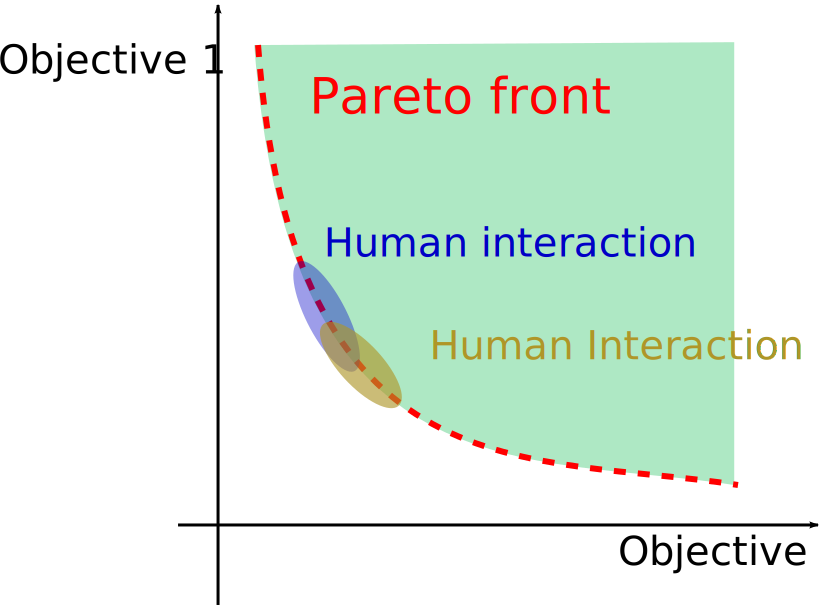
\includegraphics[width=0.4\linewidth]{./images/moo}
\caption{Interactive multi-objective optimization.}
\label{fig:moo}
\end{figure}

The task grammar from Section \ref{sec:semantic} allows two different types of information to be shared among the human supervisor and the robot:
the specific task to be performed (encoded as the verb and noun) and an adverbial qualifier on how the task should be performed.
The verb and noun specify hard constraints that must be satisfied by the solution generated by the robot's path planner.
By contrast, the adverbial modifier represents a soft constraint that the path should satisfy.

We assume that the soft constraint is fuzzy, meaning that there are several possible paths that would satisfy the soft constraint, and selecting from among these possible paths. requires an ability to balance various tradeoffs.
The Pareto front represents all possible tradeoffs, so a specific adverbial modifier does not specify a single point in the Pareto front, but rather a region of the Pareto front; any solution within this region might match the human's intent.
This is illustrated on Figure \ref{fig:moo} as  the shaded ovals.
We are developing a tool that allows a human to interactively explore this region to select a path that balances tradeoffs which satisfy human intent.
This tool bridges the difference between the way a human and a robot represent a task, and thus facilitates more effective shared mental models.
 
%With a Pareto front obtained, a human interactive decision process can be used as a posteriori method \cite{5585740}.
%The interaction process iteratively imports a human's selection in search for the most preferred solution.
%The human's selection could provide either a sub-region in the given optimal set or an improvement on the objective definition.
%It is expected that the solution set gradually converge to the most preferred one.

In terms of the robot's path planner, since the solutions generated from the multi-objective planner are Pareto optimal, information communicated from the planners to the human allow the human to refine their intent by selecting among these tradeoffs.
We introduce this interactive multi-objective optimization to solve the path planning problem modeled from a human verbal command.

Unfortunately, the solution space of a path planning problem has been greatly expanded.
This increases the difficulty of solving the multi-objective optimization problem.
Following related work on blending metric-based and topological approaches to path planning, we are developing a robot path representation using waypoints and trajectories that connect two neighboring waypoints.
This enables a two layer planning in order to enhance the planning efficiency:
\begin{itemize}
\item A coarse layer generates the waypoints.
\item A fine layer generates the trajectories between the waypoints.
\end{itemize}
The planning in both layers follow the same objectives and constraints.

When we have a shared mental model with semantic labels and a path planner that solves the multi-objective optimization problem, we can provide an efficient framework of optimized path-planners that can be flexible and adaptive to new forms of objective definitions from new scenarios and new information sources.



\bibliographystyle{plain}
\bibliography{reference}

\end{document}